\documentclass[12pt]{article}

\usepackage[T2A]{fontenc}
\usepackage[utf8x]{inputenc}
\usepackage[english, russian]{babel}
\usepackage{geometry}
\geometry{a4paper, portrait, margin=0.75in}
\usepackage{setspace}
\usepackage{graphicx}
\usepackage[normalem]{ulem}
\usepackage{float}

\begin{document}
\begin{titlepage}
    \begingroup
\fontsize{12pt}{14pt}\selectfont

\begin{center}

    Санкт-Петербургский политехнический университет имени Петра великого\\
    Институт компьютерных наук и кибербезопасности\\
    Высшая школа компьютерных технологий и информационных систем\\

    \vspace{\fill}

    \onehalfspacing
    \textbf{\huge Лабораторная работа \textnumero 12}\\
    \medbreak
    Дисциплина:\textbf{ Телекоммуникационные технологии}\\
    Тема: \textbf{ Моделирование простого передатчика и приемника с частотной манипуляцией (FSK) }\\
    \vspace{2.0cm}
\end{center}


\begin{flushright}
    \doublespacing
    Выполнил студент гр. 5130901{\textbackslash}10202 \underline{\hspace{7em}} Ануфриева В.Д.\\
    \smallskip
    Принял преподаватель \uline{\hspace{7em}}Богач Н.В. \\
    \smallskip
    "\uline{\hspace{1.5em}}" \uline{\hspace{5em}} 2024 г.\\
\end{flushright}

\vspace{\fill}

\begin{center}
    Санкт-Петербург\\
    2024 г.\\
\end{center}

\singlespacing

\pagebreak

\endgroup

\end{titlepage}

\tableofcontents
\pagebreak

\section{Постановка задачи:}

Изучить пример моделирования простого передатчика и приемника с частотной манипуляцией (FSK).  Для создания потоковой диаграммы использовать графический пользовательский интерфейс gnuradio-companion (GRC). 

\section{Ход работы:}

Используя gnuradio-companion, построим заданную блок-схему:
\begin{figure}[h]
    \centering
    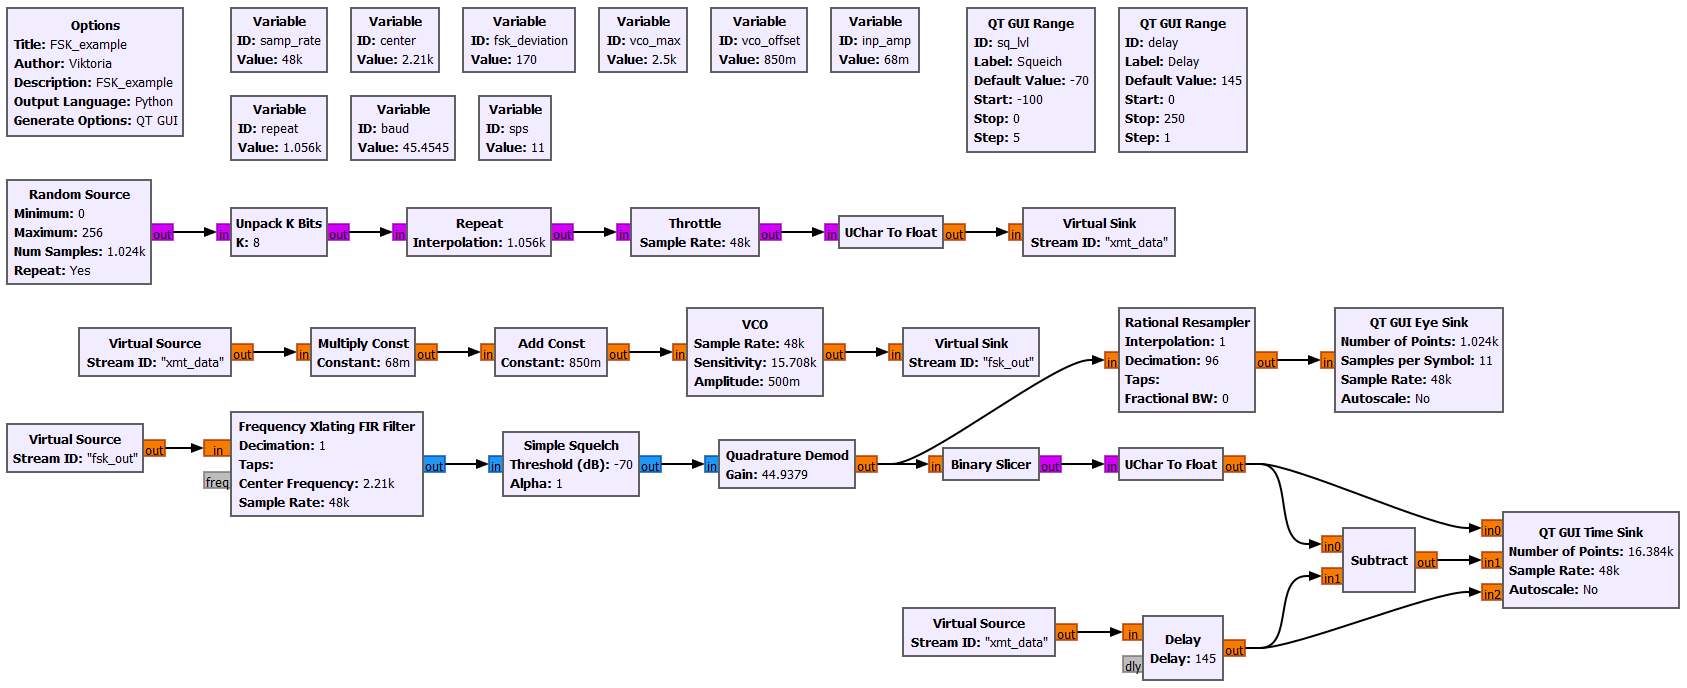
\includegraphics[width=1\textwidth]{pics/a0000-img001.png}
    \caption{Исследуемая блок-схема}
\end{figure}
Опишем основные блоки, использованные на данной схеме:

\begin{itemize}
	\item \textbf{Options} --- определяет имя файла для потоковой диаграммы, автора и т.д.
	\item \textbf{QT GUI Range} --- используется для изменения значения задержки и уровня сигнала в процессе моделирования.
	\item \textbf{Random Source} --- cлучайный источник, генерирующий байтовые значения от 0 до 255.
	\item \textbf{Unpack K Bits} --- блок выбирает K младших битов из байта и расширяет их до K байтов со значениями 0 или 1. 
	\item \textbf{Repeat} --- повторяет каждый ввод времени интерполяции.
	\item \textbf{Throttle} --- ограничитель скорости передачи данных.
	\item \textbf{UChar To Float} --- преобразовывает поток беззнаковых символов в поток чисел с плавающей запятой.
	\item \textbf{Virtual Sink} --- в сочетании с блоком Virtual Source это по сути то же самое, что протягивание провода между двумя блоками.
	\item \textbf{Virtual Source} --- в сочетании с блоком Virtual Sink это по сути то же самое, что протягивание провода между двумя блоками + источники сигналов «xmt\_data» и «fsk\_out».
	\item \textbf{Multiply Const} --- умножает входной поток на константу.
	\item \textbf{Add const} --- блок добавляет постоянное значение к каждому элементу, который проходит через него.
	\item \textbf{VCO} --- генерирует стандартные сигналы RTTY (radioteletype) частотой 2295 Гц (Отметка =1) и 2125 Гц (пробел =0).
	\item \textbf{Frequency Xlating FIR Filter} --- выполняет преобразование частоты на сигнале и одновременно понижает дискретизацию сигнала через прореживающий КИХ-фильтр. Основное использование этого блока — эффективный канализатор, позволяющий выделить узкополосную часть широкополосного сигнала без необходимости центрирования этой узкополосной части по частоте.
	\item \textbf{Simple Squelch} --- простой блок шумоподавления, основанный на средней мощности сигнала и пороге в дБ. Выход равен входу, если средний вход >= порога, и нулю в противном случае.
	\item \textbf{Quadrature Demod} --- принимает поток сложных выборок и создает поток чисел с плавающей запятой, которые представляют частотную демодуляцию.
	\item \textbf{Binary Slicer} --- разделяет значение с плавающей запятой, создавая 1-битный выходной сигнал.
	\item \textbf{Rational Resampler} --- многофазный КИХ-фильтр с рациональной повторной выборкой.
	\item \textbf{QT GUI Eye Sink} --- графический приемник на основе QT, который принимает набор сложных потоков и используется для определения правильной центральной частоты.
	\item \textbf{QT GUI Time Sink} --- графический приемник, основанный на библиотеке QT, предназначенный для отображения нескольких сигналов во временной области.
	\item \textbf{Delay} --- создаётся заданная временная задержка.
	\item \textbf{Subtract} --- производится вычитание по всем входным потокам. выход = вход\_0 - вход\_1 - ...
	\item Переменная \textbf{baud}, описывающая скорость передачи. Так как время передачи 22 миллисекунды, скорость передачи равна 1/0.022. 
	\item Переменная \textbf{repeat}, описывающая коэффициент повторяемости – (int)(samp\_rate *0.022).
	\item Переменная \textbf{vco\_offset} = 0.85 
	\item Переменная \textbf{inp\_amp} = 0.068
\end{itemize}

\textbf{Принцип работы передатчика:}
\begin{enumerate}
	\item Случайный источник генерирует байтовые значения от 0 до 255.
	\item При распаковке K битов каждый бит входных данных преобразуется в отдельный байт со значением в младшем значащем бите. 
	\item Поскольку аппаратное обеспечение не задействовано, для ограничения потока через систему используется блок Trottle.
\end{enumerate}

Блоки виртуального приемника и виртуального источника используются вместо прямого подключения для создания более чистой потоковой диаграммы. При желании можно выполнять и прямые подключения потоков.

\bigskip

\textbf{Принцип работы приёмника:}
\begin{enumerate}
	\item Частотный КИХ-фильтр сдвигает принятый сигнал так, чтобы он был центрирован вокруг center частоты – на полпути между частотами mark и space.
	\item Далее – шумоподавление, необходимое для реального приема сигналов RTTY.
	\item Блок квадратурного демодулирования выдает сигнал, который является положительным для входных частот выше нуля и отрицательным для частот ниже нуля. 
	\item Когда полученный сигнал подается на двоичный «срезатель», на выходе получается байт, равный 1 или 0. 
	\item Мы получили двоичные распакованные данные.
	\item Дополнительно добавлен приемник QT GUI Eye Sink с графическим интерфейсом QT. Он используется при настройке сигналов в реальном времени для определения правильной центральной частоты.
	\end{enumerate}

\section{Тестирование:}

Убедимся в том, что через схему проходит исходный поток битов. Для этого сравним его с входным потоком "xmt\_data". 

Диаграмма на симуляции отображает оба сигнала. Сравнив их с небольшой задержкой, (См. Рис.2) видим, что принятый сигнал отстает на некоторое количество битов, потому что цепочка передатчика и приемника имеет множество блоков и фильтров, которые задерживают сигнал. 

Для компенсации этого отставания необходимо задержать передаваемые биты на ту же величину --- используем блок Delay. Отрегулировав задержку, получаем синхронизированные потоки (См. Рис.3). Это же мы видим при вычитании одного сигнала из другого – красная кривая. В итоге правильная задержка составляет около 145.

\begin{figure}[H]
    \centering
    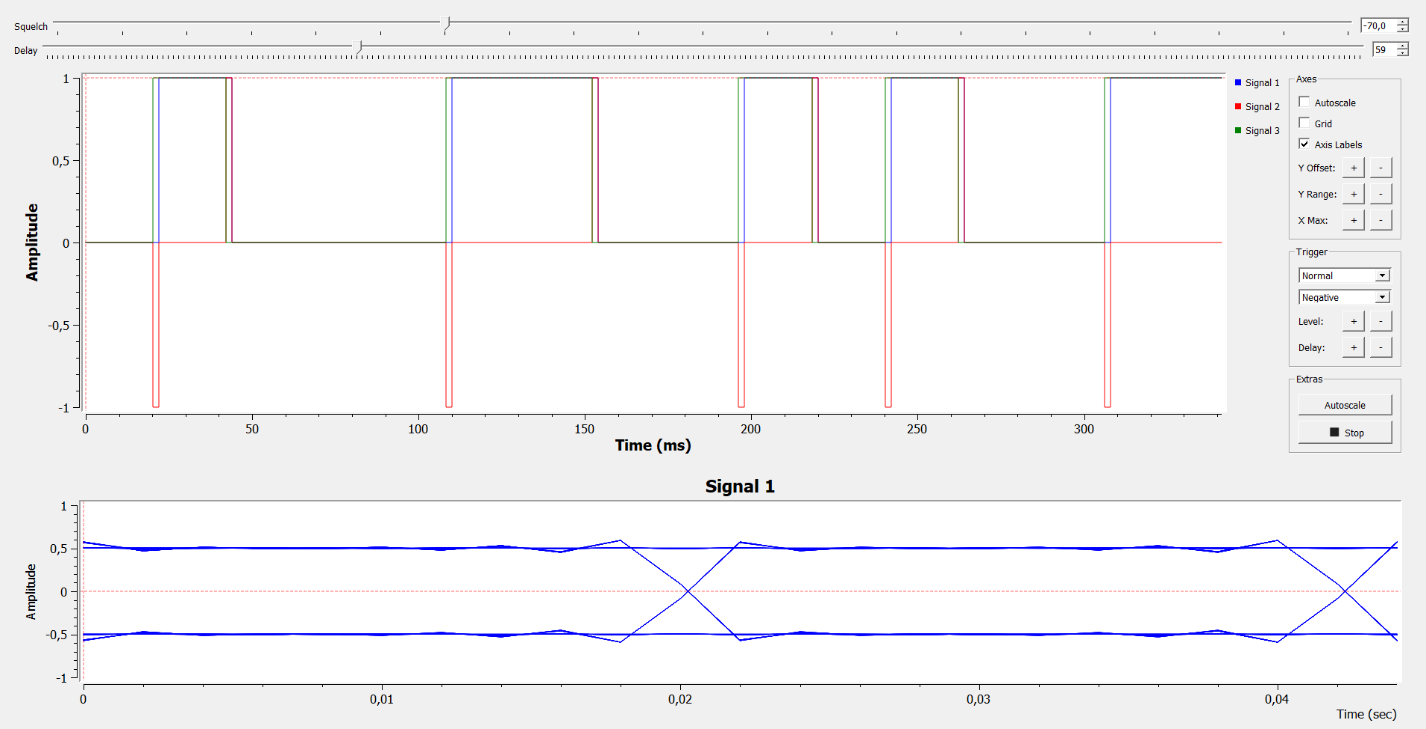
\includegraphics[width=0.8\textwidth]{pics/a0000-img002.png}
    \caption{Диаграмма с задержкой}
\end{figure}

\begin{figure}[H]
    \centering
    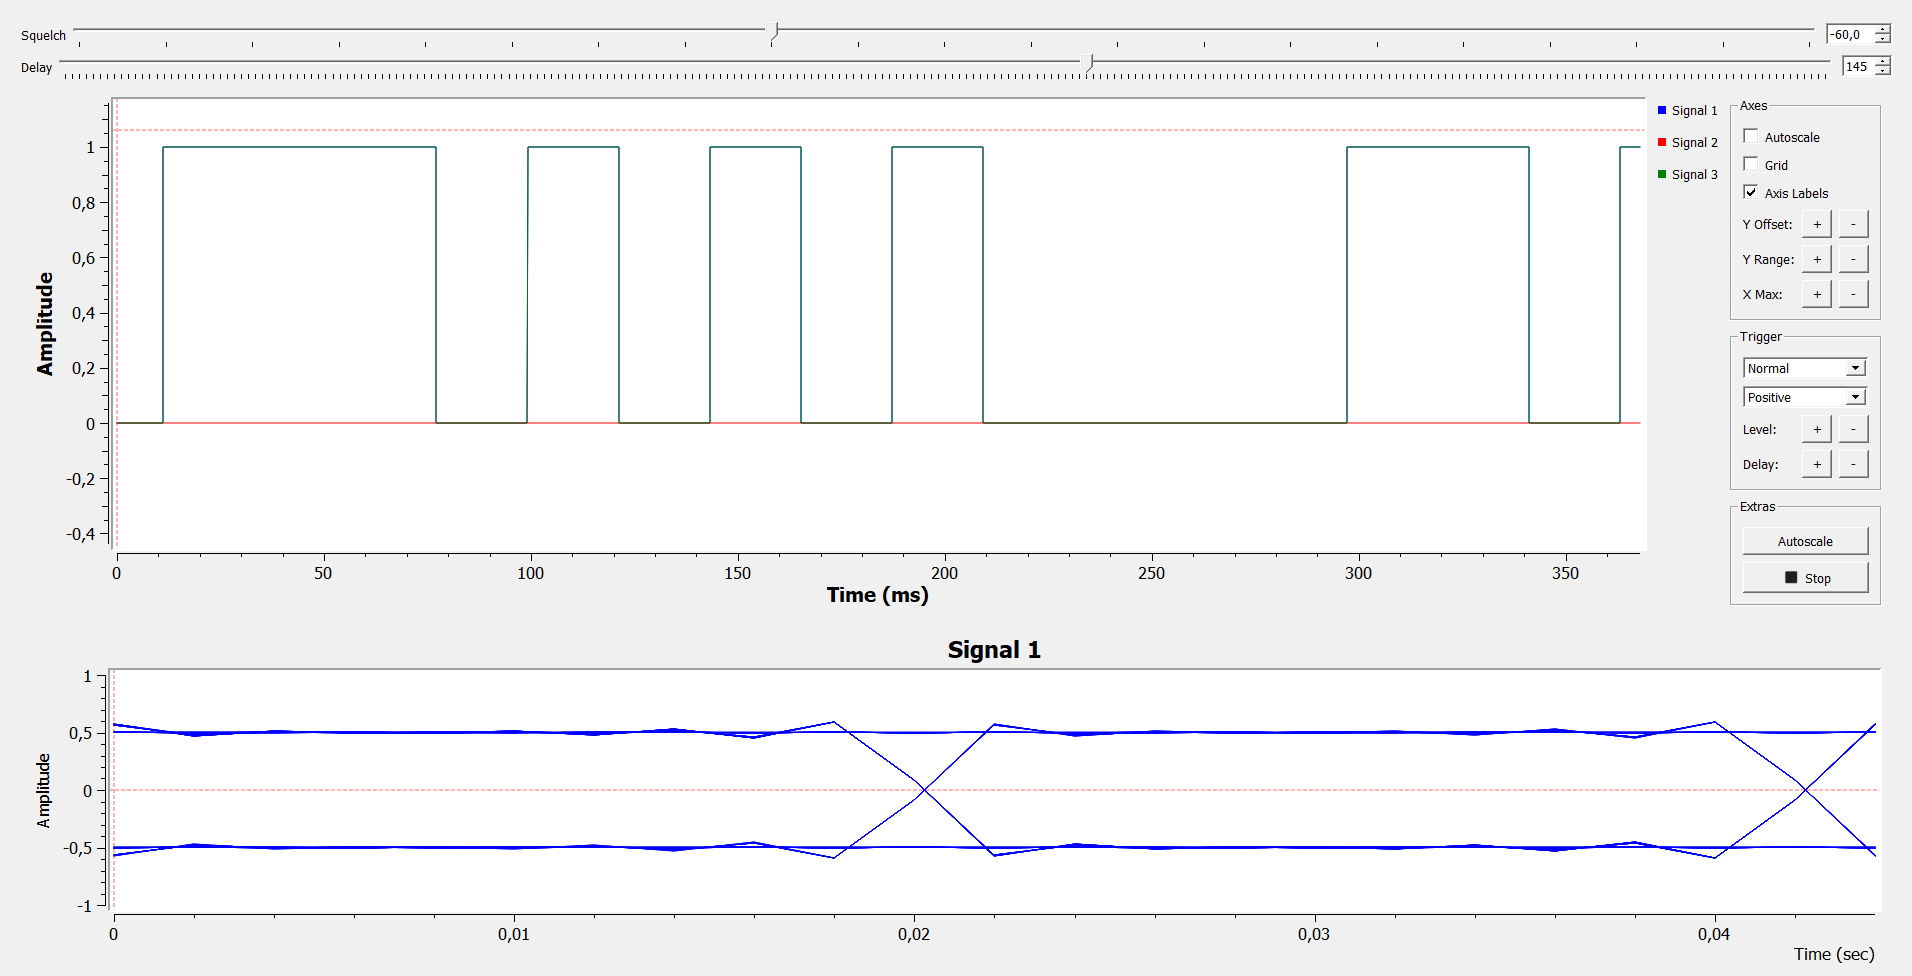
\includegraphics[width=0.8\textwidth]{pics/a0000-img003.png}
    \caption{Диаграмма со скомпенсированной задержкой}
\end{figure}

\section{Передача файлов с использованием пакетов и AFSK:}

Теперь рассмотрим пример использования FSK для отправки пакетов удаленному приёмнику. Как сказано в статье, FSK можно использовать для отправки любого содержимого данных.

Блок-схема приёмника представлена на Рис.4:

\begin{figure}[H]
    \centering
    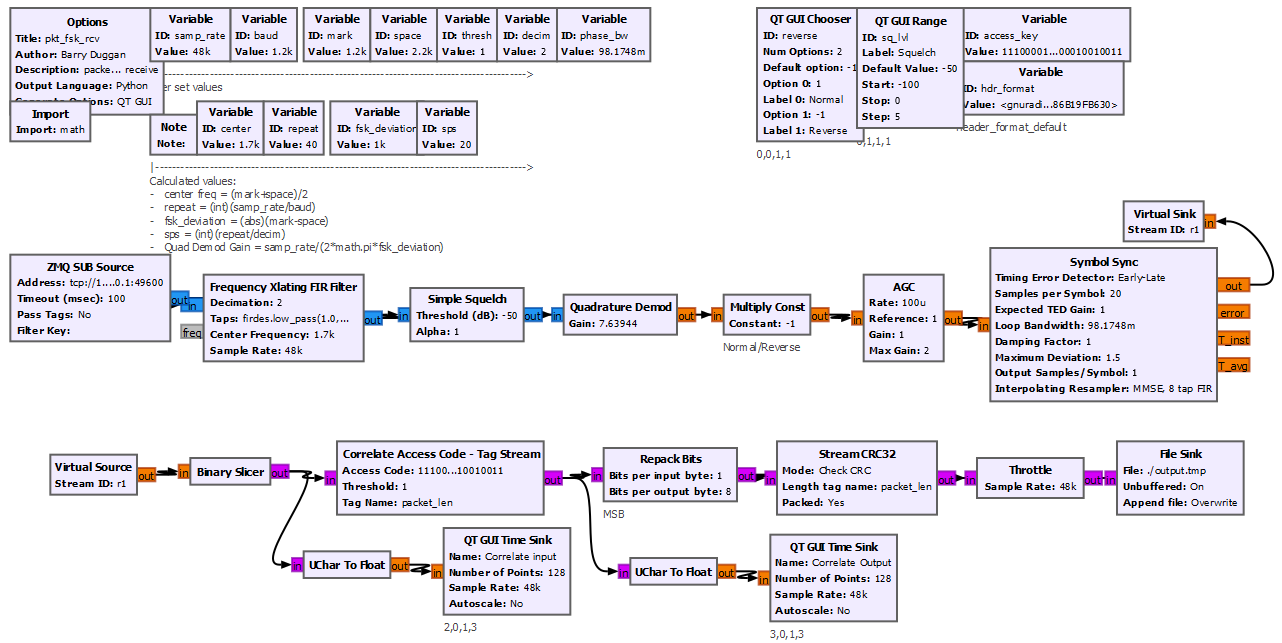
\includegraphics[width=0.8\textwidth]{pics/a0000-img004.png}
    \caption{Исследуемая блок-схема приёмника}
\end{figure}

Данная схема принимает сигнал AFSK, используя тот же частотный КИХ-фильтр и квадратурные демодулирующие блоки, что и в предыдущей схеме. Если частота Mark ниже, чем частота Space, значения 1 и 0 поменяются местами. Исправим это с использованием блока умножения константы с константой, установленной в QT GUI Chooser.

Для нормирования входного сигнала до 1, т.к. этого требует блок синхронизации символов, используем блок AGC. Как только поток битов подается в двоичный срезатель, на выходе получается распакованный байт, равный 1 или 0.

Чтобы определить начало пакета и добиться выравнивания байтов, блок корреляции потока кода доступа с тегом кода доступа обнаруживает код доступа и передает полезную нагрузку в Stream\_CRC32 для проверки допустимого CRC. Если CRC правильный, данные отправляются в File\_Sink.

\bigskip

\textbf{Передача файла:}
\medskip

Блок 'EPB: источник файла в помеченный поток' представляет собой встроенный блок Python, который заменяет блок File\_Source, блок Stream\_to\_Tagged\_Stream и части блока Burst\_Shaper. Блок Python выполняет следующие функции:
\begin{itemize}
	\item Отправка заголовка, чтобы разрешить приемнику синхронизацию.
	\item Чтение файла в виде фрагментов "Pkt\_Len".
	\item Преобразование данных в Base64, который выдает 4 байта выходных данных на каждые 3 байта входных данных.
	\item Отправка каждого фрагмента Base64 с исправленными тегами "packet\_len".
	\item Отправка заполнителя после файла, чтобы убедиться, что все буферы были сброшены.
\end{itemize}

Преамбула выглядит так: "\%", 50 заглавных букв "U", "]". Это повторяется четыре раза, чтобы приемник мог выполнить синхронизацию. Заполнитель post-файла отправляется 10 раз.

Блок-схема передатчика представлена на Рис.5:

\begin{figure}[H]
    \centering
    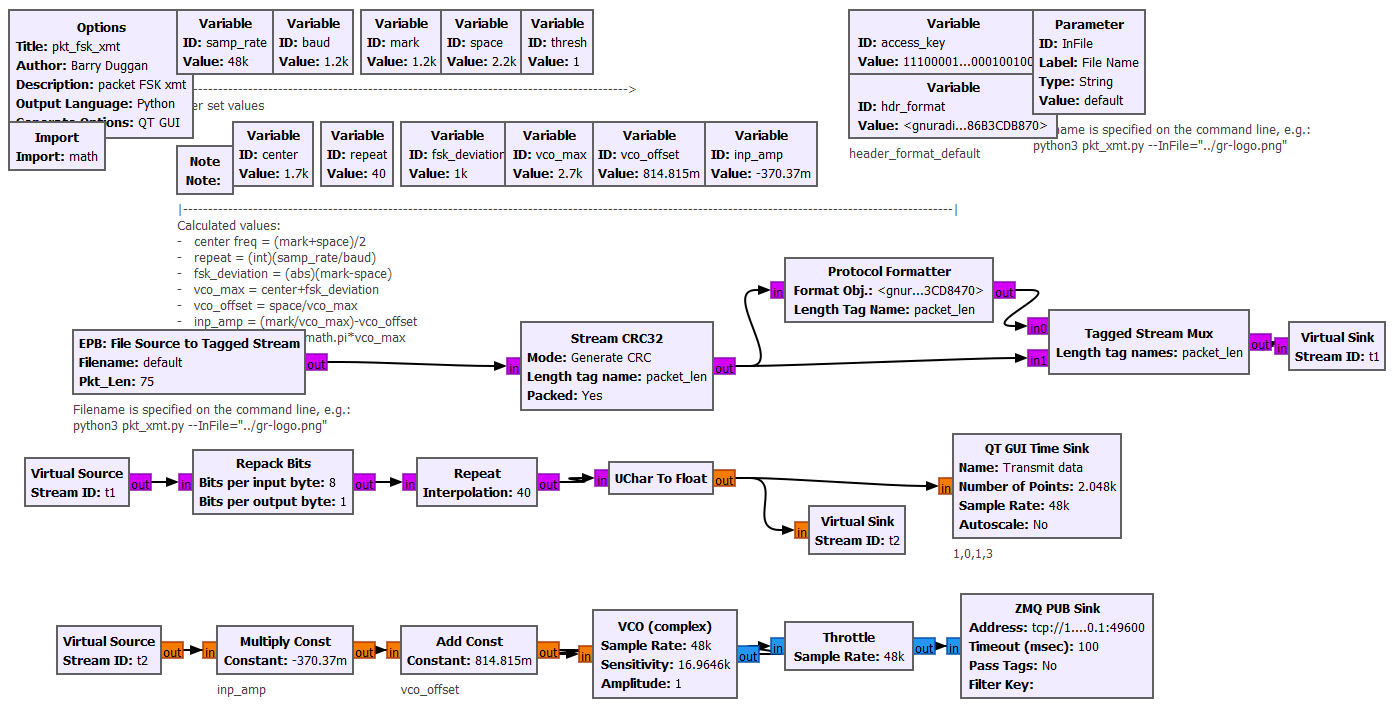
\includegraphics[width=0.8\textwidth]{pics/a0000-img005.png}
    \caption{Исследуемая блок-схема передатчика}
\end{figure}

Теперь запустим передачу пакетов с желаемым именем файла:

 python3 pkt\_fsk\_xmt.py --InFile="../gr-logo.png"
 
\begin{enumerate}

	\item В окне "pkt\_fsk\_xmt" началась передача файлов. Как сказано в статье, средняя пропускная способность составляет 150 байт в секунду. (См. Рис.6)
	
\begin{figure}[H]
    \centering
    	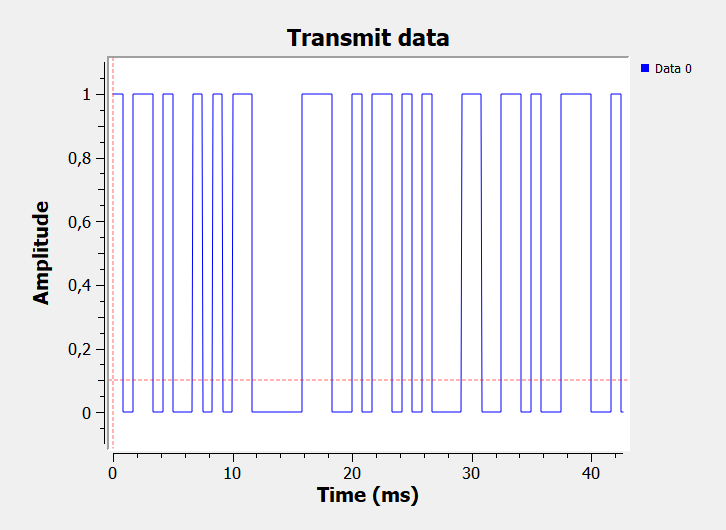
\includegraphics[width=0.8\textwidth]{pics/a0000-img006.png}
    	\caption{Диаграмма процесса передачи данных}
\end{figure}

	\item Уже через несколько секунд передача завершается, и в терминал выводятся сообщения об окончании операции: (См. Рис.7) "Конец файла" и "Окончание передачи":
	
\begin{figure}[H]
    \centering
    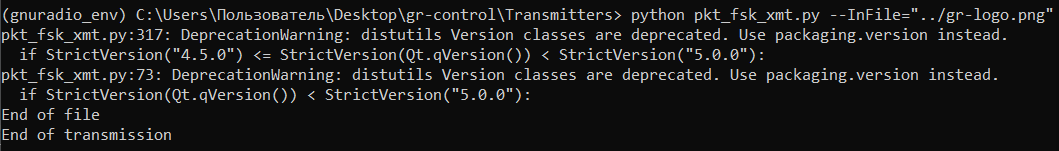
\includegraphics[width=0.8\textwidth]{pics/a0000-img007.png}
    \caption{Вывод в терминал}
\end{figure}

	\item Когда на дисплее "pkt\_fsk\_xmt" прекратилась отправка пакетов-заполнителей, дисплей "pkt\_fsk\_rcv" стал статичным, как и ожидалось: (См. Рис.8)
	
\begin{figure}[H]
    \centering
    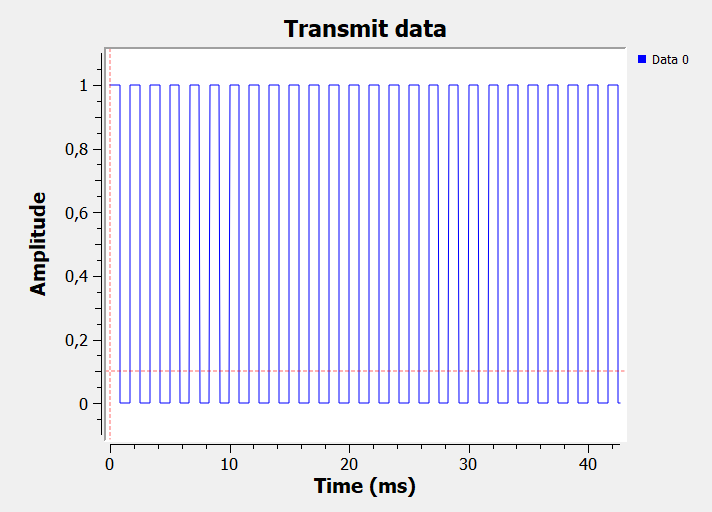
\includegraphics[width=0.8\textwidth]{pics/a0000-img008.png}
    \caption{Вывод в терминал}
\end{figure}

\end{enumerate}

Работа завершена.
\bigskip

\textbf{Удаление преамбулы и заполнителя:}
\medskip

Принятый файл сохранен в директорию "/ gr-control /Receivers /output.tmp". Этот файл содержит до четырех пакетов преамбулы, за которыми следует переданный файл с кодировкой Base64, а далее следуют пакеты заполнения.

Для удаления этих пакетов преамбулы и заполнения и декодирования текста Base64 написана программа на Python strip\_preamble.py :

python3 strip\_preamble.py output.tmp output.png

После применения команды выше, все данные из output.tmp удалены.

\end{document}


